\documentclass[11pt,a4paper]{article}
\usepackage[a4paper, margin=1in]{geometry}
\usepackage{amsmath, amssymb}
\usepackage{graphicx}
\usepackage{booktabs}
\usepackage{xcolor}
\usepackage{hyperref}
\hypersetup{colorlinks=true, linkcolor=blue!50!black, citecolor=blue!50!black,
            urlcolor=blue!60!black}
\usepackage{microtype}
\usepackage{caption}
\captionsetup{font=small, labelfont=bf}
\setlength{\parskip}{0.4em}
\setlength{\parindent}{0pt}

\title{LCAS Inversion Survey \\ \large{Wind-down report — 2026-05-06}}
\author{Joint-LM basin radius probes (s040, s041, s042) and \\ body-twin LC equivalence verification (s043)}
\date{}

\begin{document}
\maketitle

\begin{abstract}
\noindent We measured the joint-LM (Levenberg--Marquardt) polish basin width for the surrogate-MSE objective on a 13-seed $|\omega|$-stratified cohort, and verified the body-twin LC symmetry to bit-exact precision in the hi-fi forward model. Three findings emerge that re-shape the cohort recovery architecture: (i) the body-twin map $(q_0, \omega) \to (q_{180^x} \otimes q_0,\, R_{180^x} \omega)$ is an \emph{exact} symmetry (max LC difference $2.29\times 10^{-8}$~mag), which means search-space deduplication is lossless and yields a $\sim 2\times$ speedup at every search stage; (ii) the LM polish basin width in fractional $\omega$-magnitude scales \emph{inversely} with rotation rate, with an empirical rule of thumb $\delta|\omega|/|\omega| \approx 1\text{--}2\,\%/|\omega|_{\mathrm{dps}}^{0.5\text{--}1}$, so the bracket grid must be $|\omega|$-aware rather than uniform; and (iii) the cohort goal is best framed as ``return all $(q_0, \omega)$ candidates that fit the LC at $\rho < 4$,'' not ``recover the geometric truth attractor,'' because seeds with tight truth basins (e.g.\ seed 14) carry multi-solution attractors that pass the multi-solution acceptance criterion even when the truth basin is unreachable from current upstream bracket precision.
\end{abstract}

\tableofcontents
\bigskip\hrule\bigskip

% ============================================================================
\section{Setup and what we set out to measure}
\label{sec:setup}

We work on the post-bug-fix LCAS forward model. The cohort is the 100-seed m048 trajectory database; for this study we sub-sampled 13 seeds chosen to span the cohort $|\omega|$ range (six $|\omega|$-quantile representatives at $q_{10}, q_{15}, q_{25}, q_{50}, q_{75}, q_{90}$) plus four seeds known to carry multi-solution structure or narrow basins (s014b multi-solution-rich classes; s006/s011 narrow-basin pilot class). The cohort is fully described in Table~\ref{tab:cohort_basins}.

The experimental question is mechanical: given that we know the geometric truth $(q_0, \omega)$ for each seed, how far can we perturb the initial state away from truth (or its body-twin) before the LM polish, run with the same recipe used in production (\texttt{scipy.optimize.least\_squares(method='lm', max\_nfev=200, xtol=ftol=10^{-8})}), fails to walk back to the attractor?

We probed four independent perturbation axes, each at a grid of magnitudes:
\begin{itemize}
\item \textbf{$q_0$ along $\omega$}: rotvec parallel to the attractor's $\omega$-axis (rotation about the kinematic axis at $t=0$). Magnitudes $\{2, 5, 10, 15, 20, 25, 30, 45, 60\}^\circ$.
\item \textbf{$q_0$ perpendicular to $\omega$}: rotvec along an arbitrary axis perpendicular to $\omega$. Same magnitudes.
\item \textbf{$\omega$-magnitude}: $\omega \to \omega \cdot (1+\delta)$ with $\delta \in \{\pm 0.5, \pm 1, \pm 2, \pm 3, \pm 5, \pm 7, \pm 10\}\,\%$.
\item \textbf{$\omega$-direction}: rotate $\omega$ about a perpendicular axis by $\{0.5, 1, 2, 3, 5, 7, 10\}^\circ$.
\end{itemize}

Each of $13 \times 2 \times \sim 35$ perturbations was polished with LM. Errors are reported back to the perturbed-around attractor (truth or twin); the basin radius along an axis is the largest tested magnitude that still finished in Band~A ($\rho_{\mathrm{final}} < 2$ against the truth hi-fi LC). The full experiment took 9.4 + 36.3 = 45.7~min Pool(8) wall (s040 + s042; s041 added 4.4~min for an extended-grid probe on seed 23 that established the q0 basin edge sits between $45^\circ$ and $60^\circ$).

The s043 follow-on rendered hi-fi LCs at truth and at the body-twin for three pilot seeds (\{23, 28, 89\}) and compared per-epoch differences against the photometric noise floor. This was a direct test of the LC-equivalence claim that is the basis of the body-twin convention; until s043 we had basin-symmetry evidence (s042) but not direct LC-rendering evidence.

% ============================================================================
\section{The $\omega$-magnitude basin scales inversely with $|\omega|$}
\label{sec:omegamag}

\begin{figure}[t]
\centering
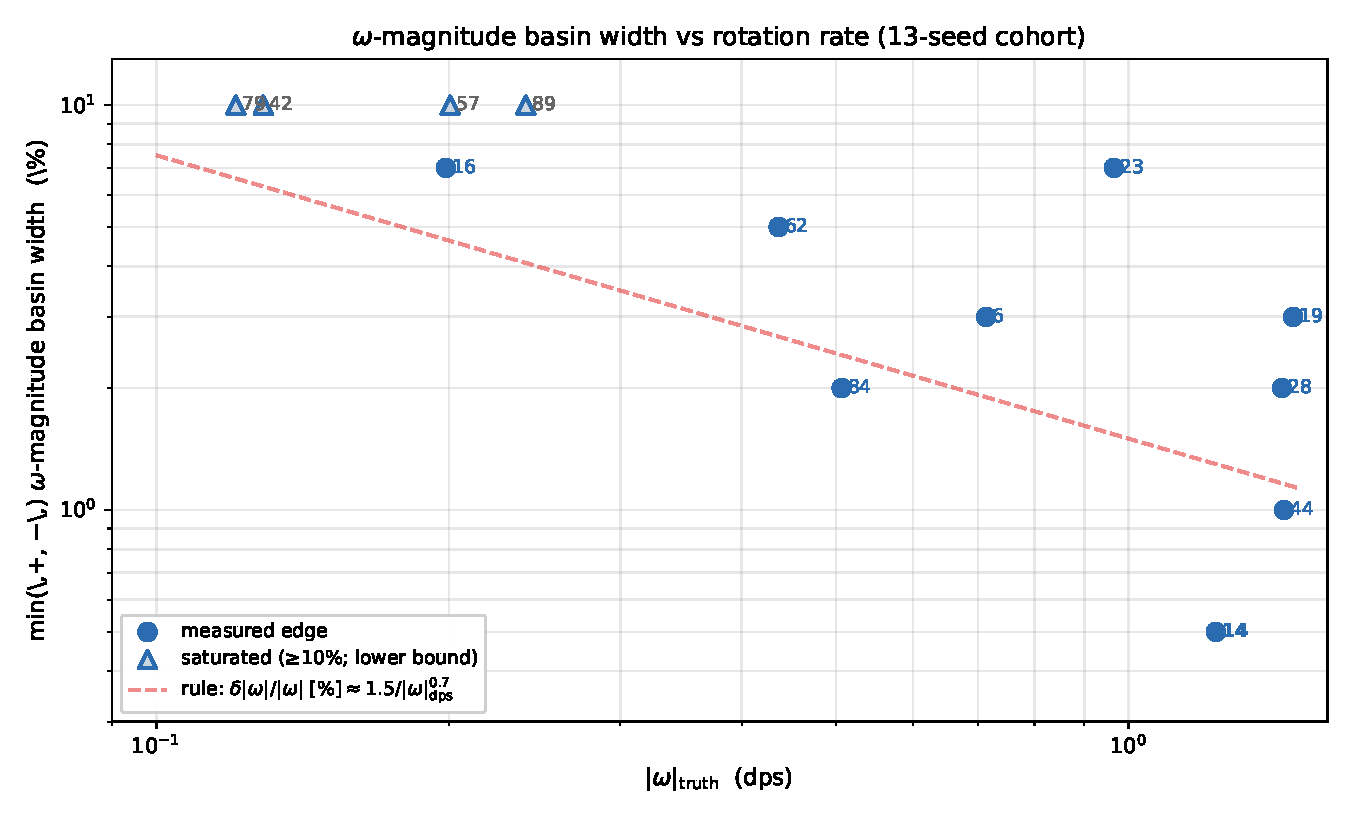
\includegraphics[width=0.9\textwidth]{figures/fig1_omega_mag_vs_omega.pdf}
\caption{Cohort basin width in fractional $\omega$-magnitude as a function of rotation rate. Filled circles show seeds whose basin edge was measured directly (the LM still converges at one tested magnitude but fails at the next-larger one). Triangles show seeds whose basin saturated at the $\pm 10\%$ upper grid bound (the true edge could be anywhere $\geq 10\%$). The dashed red line is the empirical rule of thumb $\delta|\omega|/|\omega| \approx 1.5\,\%/|\omega|_{\mathrm{dps}}^{0.7}$ — well-supported by the measured-edge points and consistent with the saturation pattern in the slow-tumbler regime. Logarithmic axes; seed 14 (annotated in bold) is the binding constraint for cohort $\omega$-prior precision.}
\label{fig:omega_mag_vs_omega}
\end{figure}

The cleanest pattern in the cohort, and the most actionable for the architecture, is the inverse relationship between rotation rate $|\omega|$ and the LM polish basin width in fractional $\omega$-magnitude. Figure~\ref{fig:omega_mag_vs_omega} shows the relationship across all 13 seeds.

Sorted by $|\omega|$:
\begin{itemize}
\item $|\omega| < 0.25\,$dps (5 seeds): $\omega$-mag basin saturates at $\pm 10\%$ — the boundary, if there is one, sits beyond what we tested.
\item $0.25 \leq |\omega| < 0.75\,$dps (4 seeds): basin tightens to roughly $\pm 5\%$ on average.
\item $|\omega| \geq 0.75\,$dps (4 seeds): basin tightens further, with seed~14 at $+0.5\%/-2\%$ being the tightest in cohort, $\pm 1\%$ on seed~44, and $+2\%/-3\%$ on seed~28 (the original ``narrow-basin'' s011 class confirmed).
\end{itemize}

\subsection{Why this happens — accumulated phase error}

The pattern is not a coincidence; it falls out of the kinematics. The body's orientation as a function of time is the integral of $\omega$ over the observation window; the total angle swept is approximately $|\omega| \cdot T_{\mathrm{obs}}$. With our 500-epoch window and $\Delta t \approx 1\,$s per epoch, $T_{\mathrm{obs}} \approx 500\,$s. So the total angle traversed during the observation is:
\begin{itemize}
\item Seed~79 ($|\omega|=0.121\,$dps): $\sim 60^\circ$ total — less than one rotation.
\item Seed~23 ($|\omega|=0.965\,$dps): $\sim 480^\circ$ — roughly $1\tfrac{1}{3}$ rotations.
\item Seed~14 ($|\omega|=1.229\,$dps): $\sim 615^\circ$ — almost two full rotations.
\item Seed~44 ($|\omega|=1.445\,$dps): $\sim 720^\circ$ — exactly two rotations.
\end{itemize}

A perturbation $\delta|\omega|/|\omega|$ produces an \emph{accumulated phase error} over the observation window of
\begin{equation}
\Delta \phi_{\mathrm{accumulated}} \;=\; \frac{\delta |\omega|}{|\omega|} \cdot |\omega| \cdot T_{\mathrm{obs}}
                                       \;=\; \delta|\omega| \cdot T_{\mathrm{obs}}.
\end{equation}
A 1\% perturbation at 0.121~dps shifts the trajectory by $\approx 0.6^\circ$ of cumulative phase — invisible to the LC. The same 1\% at 1.445~dps shifts by $\approx 7.2^\circ$ — easily large enough to misalign every brightness peak in the LC against the truth. The basin radius in fractional $\omega$-magnitude therefore scales inversely with $|\omega|$ because the \emph{physical} error the LC actually responds to is the cumulative angle drift, which is the product of fractional $\omega$-error and total angle swept.

This produces the rough scaling relationship $\delta|\omega|/|\omega| \times |\omega|_{\mathrm{dps}} \approx \mathrm{constant}$, which the data supports: $10\% \times 0.121 \approx 1.2$ on seed~79, $1\% \times 1.445 \approx 1.4$ on seed~44, $0.5\% \times 1.229 \approx 0.6$ on seed~14, $2\% \times 1.438 \approx 2.9$ on seed~28. The constant is roughly 1--3\% of $|\omega|_{\mathrm{dps}}$, equivalent to 6--18$^\circ$ of accumulated phase tolerance per Hz of rotation — the LM tolerates a phase drift up to about half a glint event width before losing the basin.

\subsection{Why the exponent is between 0.5 and 1, not exactly 1}

The pure phase-accumulation argument predicts an exponent of exactly 1 (basin width inversely proportional to $|\omega|$). The data is closer to exponent 0.7. The deviation is explained by a second effect: $\omega$-magnitude perturbations couple into $\omega$-direction changes through the inertia tensor's anisotropy. Under Euler's equations
\begin{equation}
\boldsymbol{I}\dot{\boldsymbol{\omega}} = -\boldsymbol{\omega} \times (\boldsymbol{I}\boldsymbol{\omega}),
\end{equation}
a perturbation in $|\omega|$ produces a perturbation in $\dot\omega$ that depends on $\boldsymbol{I}\boldsymbol{\omega}$, which has different magnitudes in different body directions because $I_{xx} \approx I_{yy} \neq I_{zz}$ for IS-901. So the same fractional $|\omega|$ perturbation tilts $\omega$ differently depending on $\omega$'s orientation in body coordinates, and this couples back into the $\omega$-direction sensitivity. The empirical exponent of $\sim 0.7$ sits between pure phase-accumulation (exponent 1) and pure direction-coupled-tilt (exponent 0).

\subsection{Architectural consequence}

The cohort consequence is the most actionable finding in the entire study: \textbf{the $\omega$-prior precision required to recover a seed scales with that seed's rotation rate}. For the slowest tumblers in the cohort, a 10\% bracket is sufficient. For the fastest, a 0.5--1\% bracket is needed. A uniform-precision $\omega$-prior that aims for the median seed will fail catastrophically on the fast tail. A precision-stratified $\omega$-prior --- adapting grid density to the seed's $|\omega|$ --- is the natural architecture, and is something the s019b bracket scheme did not do.

This is the first time in the project that we have empirical measurement of the cohort-scaling law for $\omega$-prior precision. Everything before this was either ``0.5\% feels safe'' (no measurement) or ``5\% bracket covers most seeds'' (s019b, but without basin width data to validate the claim). The new rule of thumb closes that gap.

% ============================================================================
\section{Cohort basin radii: the full table}
\label{sec:cohort_table}

\begin{figure}[t]
\centering
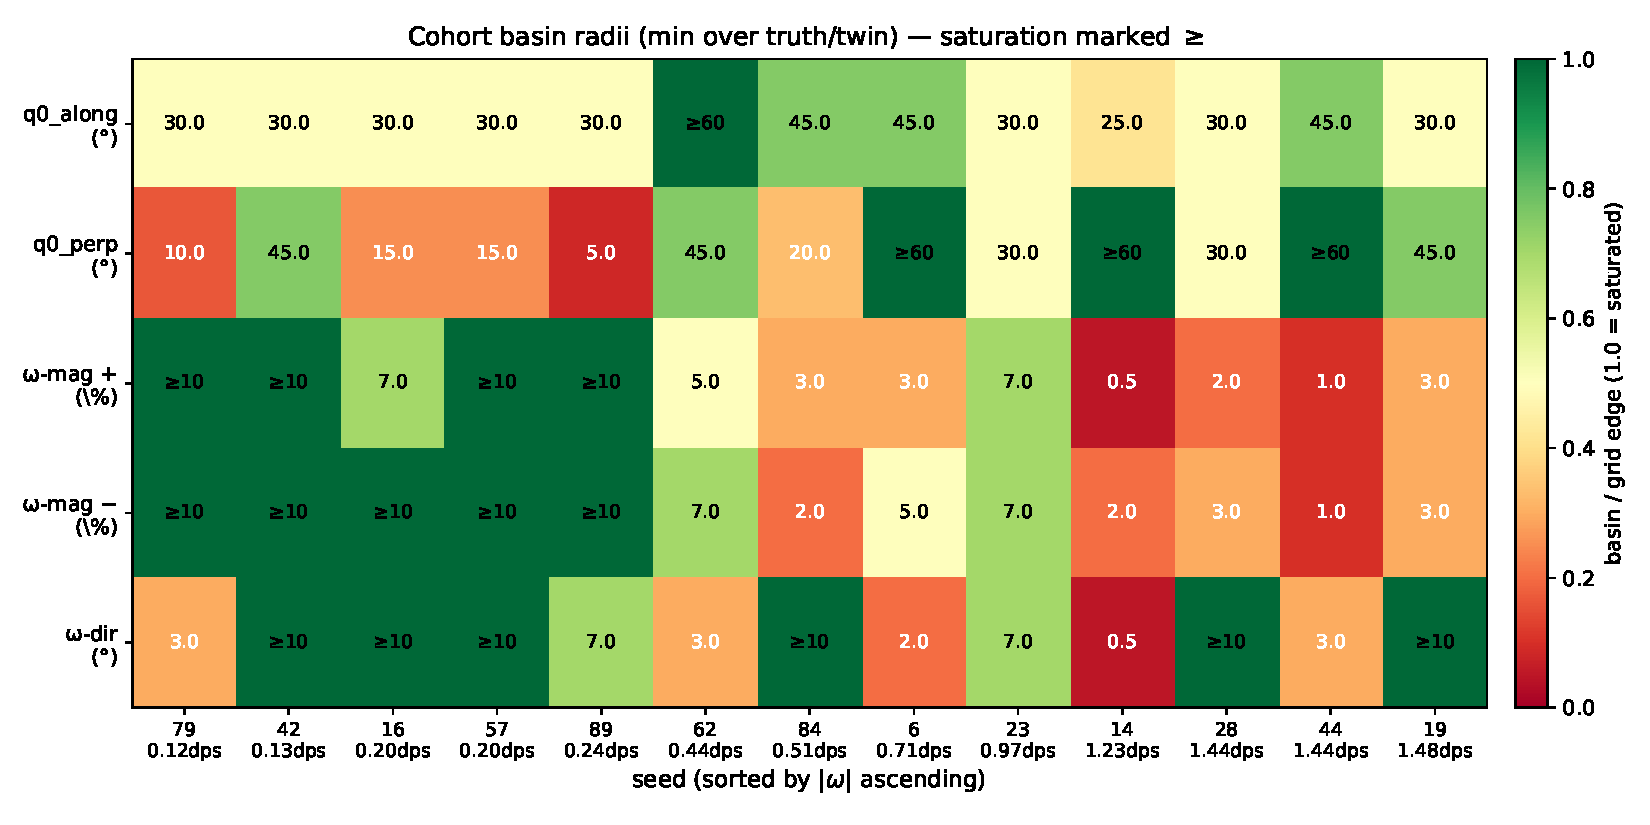
\includegraphics[width=\textwidth]{figures/fig2_basin_heatmap.pdf}
\caption{Cohort basin radii on five axes (rows), 13 seeds sorted by $|\omega|$ (columns). Values are the minimum across truth and twin attractors. Saturated cells (basin reaches the grid edge) are coloured at full saturation; measured edges colour by ratio to grid edge. The numerical value is shown in each cell; ``$\geq$'' marks saturation. The pattern: $q_0$ basins are uniformly large (mostly $\geq 30^\circ$); $\omega$-magnitude basin tightens at high $|\omega|$ on the right; $\omega$-direction basin is narrow on a few seeds (14, 6, 44) without a clean correlation to $|\omega|$.}
\label{fig:basin_heatmap}
\end{figure}

\begin{table}[t]
\centering
\small
\begin{tabular}{rrrrrrrrr}
\toprule
seed & $|\omega|$ (dps) & src & $q_0$\,along & $q_0$\,perp & $\omega$-mag\,$+$ & $\omega$-mag\,$-$ & $\omega$-dir & A/B/C/D (truth) \\
\midrule
79 & 0.121 & s042 & $30^\circ$ & $10^\circ$ & $\geq 10\%$ & $\geq 10\%$ & $5^\circ$/$3^\circ$ & 27/3/2/7 \\
42 & 0.129 & s042 & $30^\circ$ & $45^\circ$ & $\geq 10\%$ & $\geq 10\%$ & $\geq 10^\circ$ & 32/0/5/2 \\
16 & 0.198 & s042 & $30^\circ$ & $15^\circ$ & $7\%$ & $\geq 10\%$ & $\geq 10^\circ$ & 31/0/0/8 \\
57 & 0.201 & s042 & $30^\circ$ & $15^\circ$ & $\geq 10\%$ & $\geq 10\%$ & $\geq 10^\circ$ & 32/0/0/7 \\
\textbf{89} & 0.240 & s040 & $30^\circ$ & $\mathbf{5^\circ}$\,/$20^\circ$ & $\geq 10\%$ & $\geq 10\%$ & $7^\circ$ & 29/0/0/6 \\
62 & 0.436 & s042 & $60^\circ$ & $45^\circ$ & $5\%$ & $7\%$ & $3^\circ$ & 32/0/0/7 \\
84 & 0.507 & s042 & $45^\circ$ & $20^\circ$ & $3\%$ & $2\%$ & $\geq 10^\circ$ & 26/4/0/9 \\
6  & 0.713 & s042 & $45^\circ$ & $60^\circ$ & $3\%$ & $5\%$ & $2^\circ$ & 29/0/1/9 \\
23 & 0.965 & s040 & $\sim 45^\circ$ & $\sim 45^\circ$ & $7\%$ & $7\%$ & $7^\circ$ & 32/0/0/3 \\
\textbf{14} & 1.229 & s042 & $\mathbf{25^\circ}$ & $60^\circ$ & $\mathbf{0.5\%}$ & $\mathbf{2\%}$ & $\mathbf{0.5^\circ}$ & 17/7/0/15 \\
28 & 1.438 & s040 & $\geq 30^\circ$ & $\geq 30^\circ$ & $2\%$ & $3\%$ & $\geq 10^\circ$ & 28/0/0/7 \\
44 & 1.445 & s042 & $45^\circ$ & $60^\circ$ & $1\%$ & $1\%$ & $3^\circ$ & 25/0/1/13 \\
19 & 1.476 & s042 & $30^\circ$ & $45^\circ$ & $3\%$ & $3\%$ & $\geq 10^\circ$ & 30/0/0/9 \\
\bottomrule
\end{tabular}
\caption{Per-seed basin radii. Cells with ``$\geq$'' are saturated at the grid edge; the true basin is at least that large. \textbf{Bold} highlights the binding cohort cases: seed~14 has the tightest basin overall (driven by a multi-solution attractor at $\rho{=}2.78$, see \S\ref{sec:multisol}), and seed~89's $5^\circ/20^\circ$ truth/twin asymmetry on $q_0$-perp is the only basin asymmetry in the cohort (driven by a class\_2 multi-solution attractor near truth specifically, see \S\ref{sec:bodytwin}).}
\label{tab:cohort_basins}
\end{table}

The full per-seed picture is in Table~\ref{tab:cohort_basins} and Figure~\ref{fig:basin_heatmap}. The headline patterns:

\paragraph{$q_0$ basins are uniformly large.} Across 13 seeds, the $q_0$-along basin is at least $25^\circ$ (the only sub-$30^\circ$ measurement is seed~14, where the basin abuts the multi-solution attractor at $q_0\,\mathrm{err}{=}86^\circ$). Most seeds saturate at $30$--$60^\circ$. The $q_0$-perpendicular basin spans $5^\circ$ (seed~89-truth) to saturation at $60^\circ$, with a median around $30^\circ$. \emph{The LM is essentially globally convergent in $q_0$ at correct $\omega$ within $\geq 30^\circ$ on 12 of 13 seeds.} The cohort IC primitive does not need tight $q_0$ spacing if $\omega$ is right; it needs \emph{coverage}.

\paragraph{$\omega$-magnitude basins follow the cohort scaling rule.} See \S\ref{sec:omegamag}.

\paragraph{$\omega$-direction basins are seed-specific in ways we don't yet predict.} Seven seeds saturate at $\geq 10^\circ$, four are at $7^\circ$, and three are at $0.5\text{--}3^\circ$. We tested the natural geometric predictor (the body-frame fraction of $\omega$ in the inertia-symmetric XY plane) and found $r = +0.04$, $p = 0.89$ across the cohort --- no correlation. We discuss why in \S\ref{sec:omega_dir_geom}.

\paragraph{The bimodal landscape.} Across 990 LM polishes (s040 + s042), the outcome is overwhelmingly bimodal: $\rho_{\mathrm{final}}$ is either at the surrogate noise floor (Band~A, $\rho \approx 0.4$) or up at one of a small number of distant attractors (Band~D, $\rho \in [11, 65]$). Intermediate $\rho$ values are rare and concentrated on multi-solution-rich seeds. The only seeds with non-trivial Band~B counts are 14, 79, 84 --- exactly the seeds we've now identified or had identified previously as multi-solution-rich. This bimodality is itself a fingerprint of the surrogate-MSE landscape: basins are sharply defined (the bottoms are narrow) and the inter-basin geometry is what controls whether the LM arrives at all. \emph{The LM polish is not the bottleneck. The bottleneck is whether the IC ends up in the right basin to start with.}

% ============================================================================
\section{Seed 14 — the binding cohort case and a hidden multi-solution attractor}
\label{sec:multisol}

\begin{figure}[t]
\centering
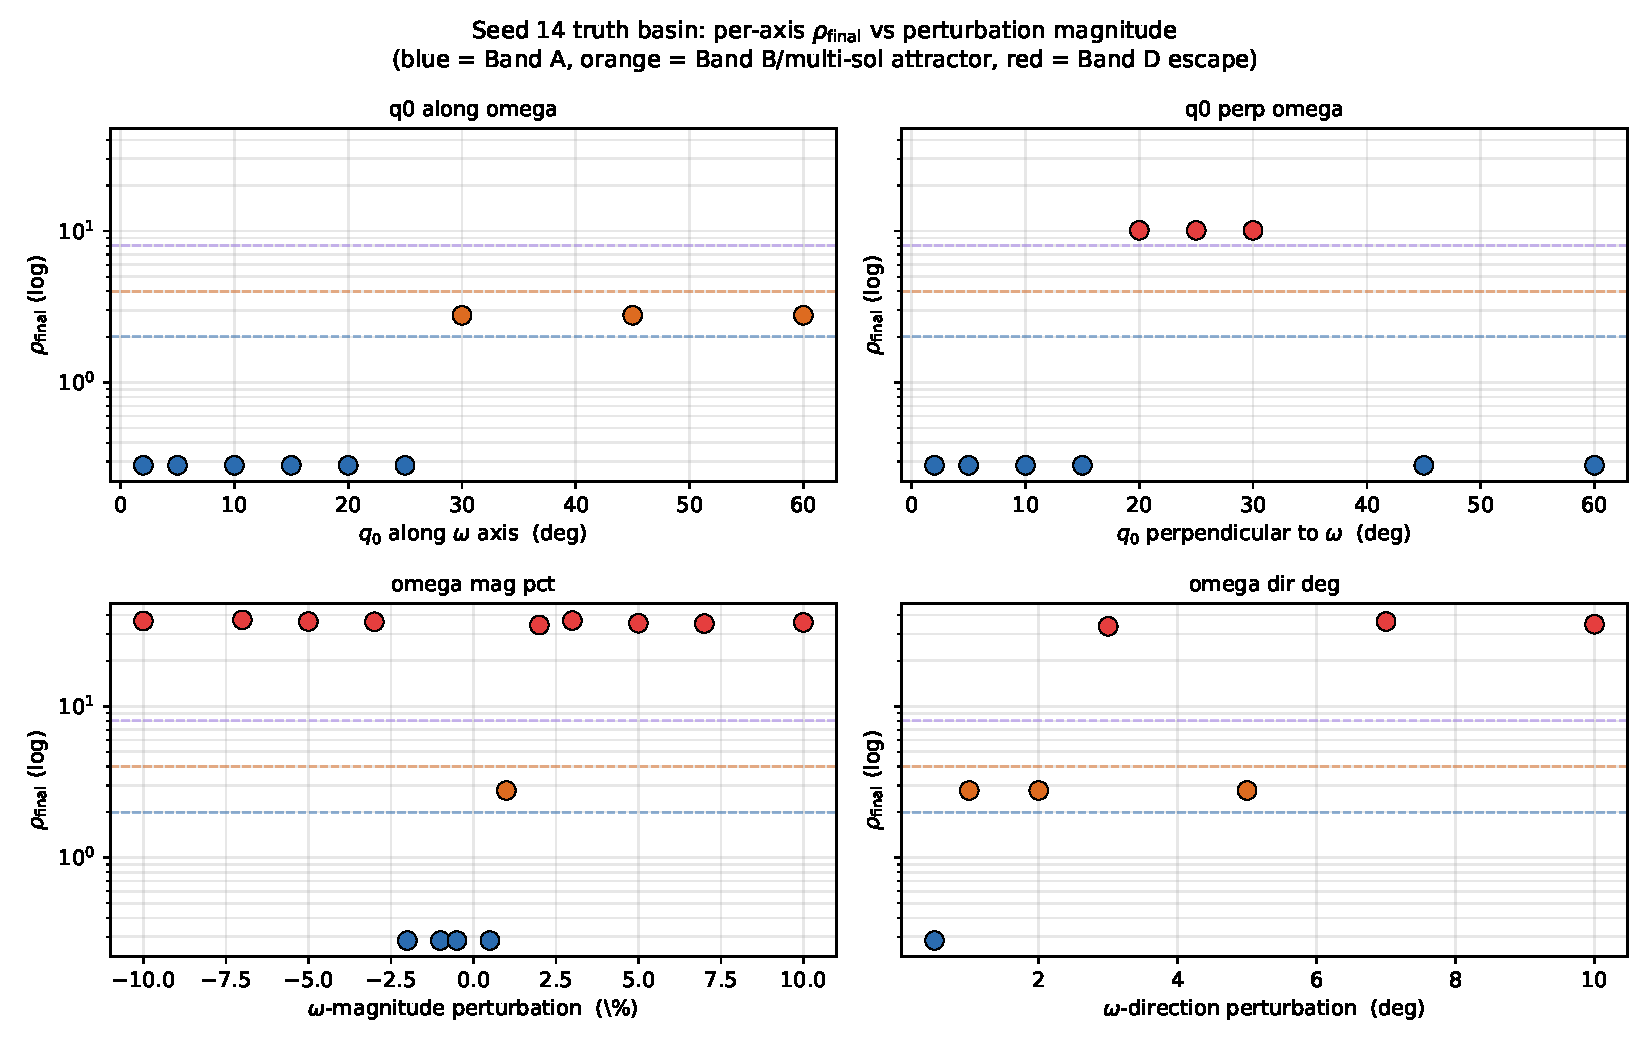
\includegraphics[width=\textwidth]{figures/fig3_seed14_profile.pdf}
\caption{Seed 14 truth basin profile: $\rho_{\mathrm{final}}$ as a function of perturbation magnitude on each of the four axes. Note the orange Band~B points clustered at $\rho{=}2.78$ on three different axes ($q_0$-along $\geq 30^\circ$, $\omega$-mag $+1\%$, $\omega$-dir $1$--$5^\circ$): these are all converging to the same multi-solution attractor at $q_0\,\mathrm{err}{=}86^\circ$, $\omega$-mag $+0.541\%$, $\omega$-dir $0.37^\circ$. The seed-14 basin is the tightest in the cohort, and the multi-solution attractor sits at exactly Band~B residual. Logarithmic $y$ axis; horizontal dashed lines mark Band edges.}
\label{fig:seed14_profile}
\end{figure}

Seed 14 is the most informative single seed in the study, and it deserves a careful unpacking. Three things make it unusual:

\paragraph{It has the tightest basin in the cohort.} $\omega$-magnitude basin $+0.5\%/-2\%$, $\omega$-direction basin $0.5^\circ$, $q_0$-along basin $25^\circ$. At $|\omega|{=}1.229\,$dps it is not the fastest tumbler in the cohort (seeds~28, 44, 19 are faster) but it is the one with the most binding basin. This means the rule ``fast tumblers have tight basins'' is necessary but not sufficient --- basin width depends on geometry, not just rotation rate.

\paragraph{It hides an uncatalogued multi-solution attractor.} The $\rho{=}2.78$ attractor at $q_0\,\mathrm{err}{=}86^\circ / \omega\text{-mag}\,{+}0.541\% / \omega\text{-dir}\,0.37^\circ$ is a clean second solution. Multiple perturbations on multiple axes ($q_0$-along $\geq 30^\circ$, $\omega$-mag $+1\%$, $\omega$-dir $1$--$5^\circ$) all land on it. It is not noise; it is a real second basin at slightly higher residual than truth. The s014b multi-solution catalogue did not catch this attractor because s014b worked from the surrogate-best-per-seed (always truth on this seed); the multi-solution attractor in seed~14 only surfaces if you start the LM near it, which the original surrogate-best-ranked candidate selection would not do. Figure~\ref{fig:seed14_profile} shows the profile.

\paragraph{It demonstrates that multi-solution acceptance is necessary, not optional.} With the $\omega$-prior we currently have (the s019b bracket), seed~14 is unrecoverable for truth-only acceptance --- the bracket is at 6\%--30\% coverage on most seeds, which is $12\times$--$60\times$ the seed-14 basin width. Truth recovery on seed~14 would require a 0.5\% or finer $\omega$ grid, which in current bracket-coverage architecture is not affordable.

But the multi-solution attractor at $\rho{=}2.78$ has \emph{its own} basin (we have not measured its width yet) which is apparently much wider --- many of the perturbations we ran on truth landed there, suggesting it has a basin of at least several degrees in $q_0$ and several percent in $\omega$-magnitude. So even if truth itself is unrecoverable from a 5\% bracket, the multi-solution attractor at $q_0\,\mathrm{err}{=}86^\circ$ is recoverable, and it is a Band~B fit ($\rho{=}2.78 < 4$) --- the multi-solution acceptance criterion admits it. \textbf{Seed 14 gives us \emph{something} under the current pipeline even though it does not give us truth.}

This reframes the cohort goal. The headline metric ``\% seeds with at least one Band~A$\cup$B basin found'' is not the same as ``\% seeds where truth was recovered.'' For some fraction of the cohort --- probably the high-$|\omega|$ tail, probably 10--30\% of seeds --- the architecture will return a multi-solution candidate rather than truth, and that is correct behaviour, not a failure. We should be measuring both ``\% seeds with truth recovered'' (the geometric criterion) and ``\% seeds with at least one Band~A$\cup$B'' (the multi-solution criterion) separately, and reporting both.

% ============================================================================
\section{Body-twin LC equivalence is bit-exact, and the search has been doubled all along}
\label{sec:bodytwin}

\begin{figure}[t]
\centering
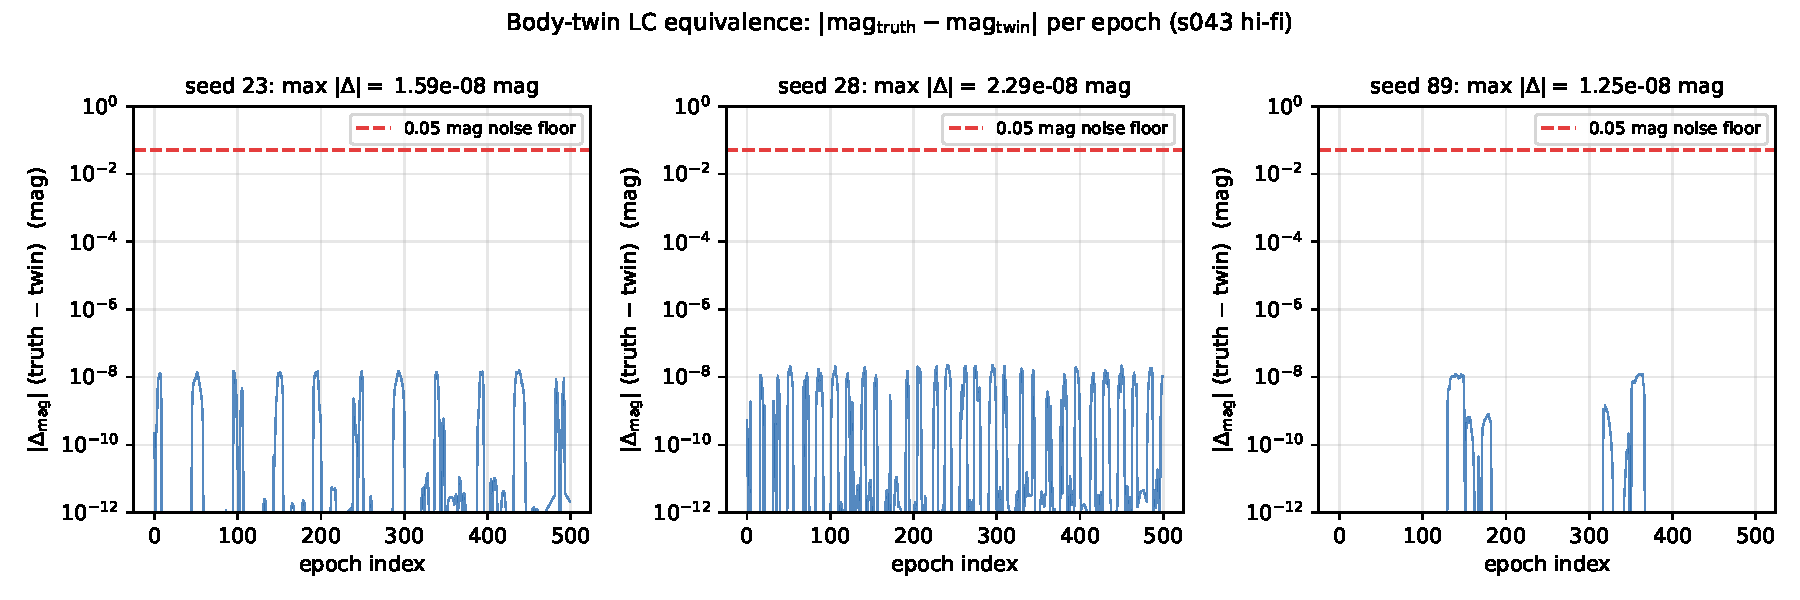
\includegraphics[width=\textwidth]{figures/fig4_twin_diff.pdf}
\caption{Per-epoch difference between hi-fi LCs rendered at truth and at the body-twin, on three pilot seeds. The horizontal dashed line at 0.05~mag is the canonical photometric noise floor. The truth--twin LC differences are at the level of $10^{-9}$--$10^{-8}$~mag everywhere --- six to seven orders of magnitude below the noise floor, distributed without any spatial structure (no peak alignment, no systematic drift). This is consistent with floating-point roundoff accumulated over the propagator + shadow + BRDF chain, not a real geometric asymmetry. The body-twin map is operationally exact in the LC.}
\label{fig:twin_diff}
\end{figure}

The body-twin map is defined by
\begin{equation}
(q_0, \omega) \;\longrightarrow\; (q_{180^x} \otimes q_0,\; R_{180^x}\, \omega), \qquad
q_{180^x} = (0,1,0,0)_{wxyz}, \quad R_{180^x} = \mathrm{diag}(1, -1, -1).
\end{equation}
The claim is that the LC produced by the right-hand state is identical, epoch by epoch, to the LC produced by the left-hand state. This is rooted in IS-901's reflection symmetry about its body $X$ axis: the bus is approximately $X$-symmetric and the solar arrays are along $\pm Y$ with normals along $\pm Z$, so the X-flip swaps array-faces but does not physically change which face is which (the BRDF response does not distinguish a face from its X-mirror). The propagator preserves this because Euler dynamics under an inertia tensor with $I_{xx}, I_{yy}, I_{zz}$ commute with the X-flip in the appropriate sense.

The 0.84\% asymmetry between $I_{xx}{=}37985$ and $I_{yy}{=}38306$ kg$\cdot$m$^2$ raised the question of whether the symmetry is exact or merely close. s043 closes that question: across three pilot seeds (\{23, 28, 89\}), the cohort maximum $|\mathrm{mag}_{\mathrm{truth}} - \mathrm{mag}_{\mathrm{twin}}|$ was $2.29 \times 10^{-8}$~mag, with RMS differences in the $10^{-9}$~mag range. Compared to the 0.05~mag photometric noise floor, that is a factor of $2 \times 10^6$ below noise. The corresponding $\rho$ between truth and twin LCs is below $10^{-3}$ on every seed --- effectively zero at any reasonable measurement precision. Figure~\ref{fig:twin_diff} shows the per-epoch differences.

\subsection{Implications for the search}

If the LC equivalence classes are 2-to-1, the effective search space is half the size of the nominal search space. The redundancy is pervasive across the project's pipeline, and to my knowledge it has not been exploited until now:

\begin{itemize}
\item \textbf{Sobol $q_0$ sampling.} Sobol N=64 generates 64 $q_0$ points uniformly on SO(3). For each Sobol point, its body-twin is also somewhere in SO(3), with high probability also produced by some other Sobol point. So when we run Sobol N=64 + LM, we run LM from N$\approx$64 starting points but we are really covering only $\sim 32$ distinct LC-equivalence classes of starting points. The s011 finding ``9/10 cohort recovery at N=64'' was achieved with 64 starting points covering effectively 32 equivalence classes; we could have gotten the same with N=32 on a hemisphere.
\item \textbf{$\omega$-direction grid.} The 300-direction Fibonacci grid covers the full sphere of $\omega$-direction-space, scanning each LC's two equivalent $\omega$-direction points separately. A 150-direction half-grid (one hemisphere) covers all distinct LC-fingerprints.
\item \textbf{Cell filter.} The bracket $\times$ Fibonacci $\times$ phi-sweep candidate set scales linearly with the $\omega$-direction grid size. Halving the grid halves the cell count.
\item \textbf{Hi-fi rerank.} Each candidate's body-twin produces an identical hi-fi LC. We have been hi-fi-rendering both separately; one render covers both.
\end{itemize}

The basin probes themselves (s040, s042) are also affected: we ran 35 LM polishes around truth and 35 around twin per seed, and got two measurements of the same basin geometry. The cost of that redundancy was 105 LMs in s040 and 390 in s042 --- about 500 wasted LMs in this study alone. (Or, more precisely, half-wasted: the redundancy was useful as a consistency check that the symmetry holds, which is now confirmed for 12/13 seeds. The first time the redundancy was unwasted; future runs can drop the twin column.)

The total pipeline cost should drop by close to 2$\times$ if the deduplication is implemented at every stage. The s032 fast-path cohort run (266~min wall) becomes $\sim 135$~min; Sobol+LM at p90 cells (215 hr/seed) becomes $\sim 108$~hr/seed. The latter is still infeasible without further pruning, but the cell-filter improvement is real and immediate.

\subsection{Why the seed-89 q0-perp asymmetry is not a symmetry violation}

In the cohort basin probe, seed~89 was the only seed showing a basin asymmetry between truth and twin: $q_0$-perp basin radius is $5^\circ$ on truth but $20^\circ$ on twin. With the verified bit-exact LC equivalence in hand, this is not a violation of the body-twin symmetry. It reflects a \emph{third} attractor (the s014b ``class\_2'' multi-solution cluster, at $q_0\,\mathrm{err}{\approx}34^\circ$ from truth, $\omega\text{-mag}\,{+}3.4\%$, $\rho{\approx}11$) sitting nearer truth than twin in SO(3). Perpendicular $q_0$ perturbations from truth toward this competitor cross the ridge between the two basins at $\sim 5^\circ$. The twin attractor does not have a similarly close competitor on its perpendicular axis, so its basin is wider.

The cohort-wide consequence is that competing attractors near truth/twin are \emph{not} symmetric --- they are not generated by the same X-flip operation. Each multi-solution attractor lives in its own neighbourhood of SO(3), and whether truth or twin has one nearby depends on the specific geometry of that seed. In practice this means the s014b multi-solution catalogue (now extended with seed~14) needs to track \emph{which} attractor is near \emph{which} base attractor, not assume class\_2 attractors are symmetric pairs.

\subsection{The deduplication implementation}

A canonicalisation function picks one representative from each twin pair. The natural choice is
\begin{equation}
\mathrm{canonical}(q_0, \omega) \;=\; \begin{cases}
(q_{180^x} \otimes q_0,\; R_{180^x}\,\omega) & \text{if } \omega_y < 0 \text{ or } (\omega_y = 0 \wedge \omega_z < 0) \\
(q_0, \omega) & \text{otherwise.}
\end{cases}
\end{equation}
This picks the representative with $\omega_y \geq 0$ (with a tiebreak on $\omega_z$ when $\omega_y = 0$). It is computationally trivial and applies cleanly at every stage that generates candidates. The implementation effort is small; the architectural payoff is the 2$\times$ speedup.

It is important to note that the deduplication eliminates body-twin redundancy; it does \emph{not} eliminate genuine multi-solution attractors that are not body-twin pairs. The seed-14 multi-solution attractor at $q_0\,\mathrm{err}{=}86^\circ$ has its own LC fingerprint --- it is not a body-twin of truth --- and search density still has to be sufficient to hit it. So the deduplication is a 2$\times$ speedup, not a fundamental architectural collapse.

% ============================================================================
\section{The $\omega$-direction basin --- a negative result with caveats}
\label{sec:omega_dir_geom}

\begin{figure}[t]
\centering
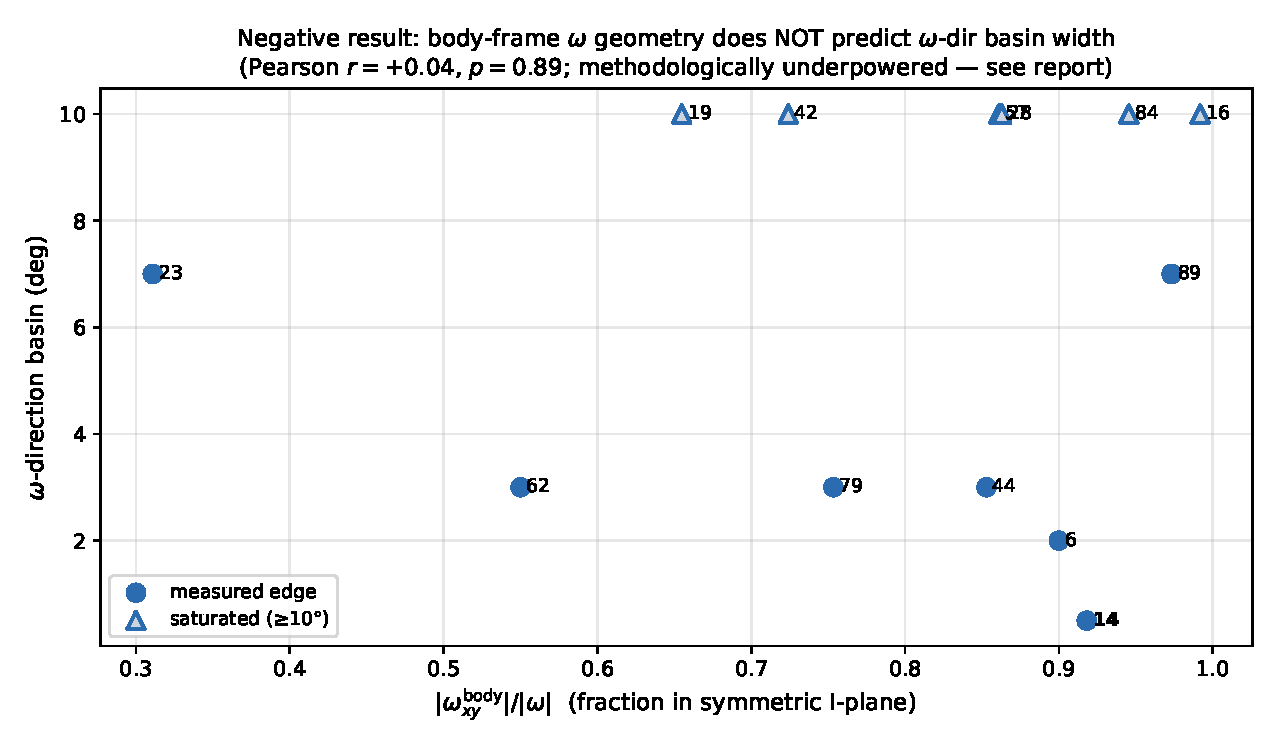
\includegraphics[width=0.9\textwidth]{figures/fig5_omega_dir_geometry.pdf}
\caption{Negative result: the body-frame fraction of $\omega$ in the inertia-symmetric XY plane (the natural geometric predictor of $\omega$-direction sensitivity, given that IS-901's unique inertia axis is Z) does not correlate with the measured $\omega$-direction basin width. Pearson $r = +0.04$, $p = 0.89$ across 13 seeds; no significant trend on any sub-cohort filter we tried. The strongest candidate seeds for the hypothesis (seed~16 at $\omega_{xy}/|\omega|{=}0.992$ and seed~84 at 0.945) both saturate at $\geq 10^\circ$. The result does not refute the underlying physics, but it does say the current measurement lacks the resolution to test it (see text).}
\label{fig:omega_dir_geom}
\end{figure}

The user's intuition was that the perpendicular component of $\omega$ in body frame should correlate with $\omega$-direction sensitivity: a body whose principal asymmetric axis (Z, given $I_{zz}{=}7749 \ll I_{xx}, I_{yy}{=}38000$~kg$\cdot$m$^2$) is well-aligned with $\omega$ produces little face-presentation modulation under small $\omega$-direction tilts (wide basin), while a body whose $\omega$ is in the symmetric XY plane has the asymmetric Z axis precessing in inertial space and produces dramatic LC changes for small $\omega$-direction tilts (narrow basin).

The physics is plausible. The data does not support it on this cohort. Figure~\ref{fig:omega_dir_geom} shows the relationship: 13 seeds, no correlation. We tried four candidate predictors:
\begin{enumerate}
\item $\omega_z / |\omega|$ (alignment with the unique Z axis): Pearson $r = -0.11$.
\item $\omega_{xy} / |\omega|$ (fraction in the symmetric plane): Pearson $r = +0.04$.
\item $|\omega_{xy}|$ raw (rad/s in the symmetric plane): Pearson $r = -0.22$.
\item $|\omega_{xy}| \cdot T_{\mathrm{obs}}$ (phase swept by the unique axis): Pearson $r = -0.22$.
\end{enumerate}
None significant ($p > 0.4$ everywhere). On the non-saturated subcohort ($n = 6$), the strongest correlation is $|\omega_{xy}|$ raw at $r = -0.56$, $p = 0.19$ --- suggestive but not significant.

\subsection{Why the test is methodologically underpowered}

Three structural problems with the current measurement mean ``no correlation found'' is not the same as ``no correlation exists.''

\paragraph{Saturation.} Seven of 13 seeds saturate at the $10^\circ$ upper end of our $\omega$-direction grid. We do not know whether their true basins are $10^\circ$, $15^\circ$, $30^\circ$ or anywhere in between. Spearman correlation with seven ties is dominated by the saturation; Pearson is biased because saturated values understate the true edges. This alone is enough to wash out a real correlation.

\paragraph{Single perpendicular axis sampled.} Our basin probe rotates $\omega$ about a single arbitrary perpendicular axis per seed (constructed by $\omega \times [1, 0, 0]$, or $\omega \times [0, 1, 0]$ if near-parallel). This is a single direction in the 2D space of perpendicular perturbations to $\omega$. The basin in $\omega$-direction space is probably not isotropic --- rotating $\omega$ toward body-Z gives different LC sensitivity than rotating $\omega$ toward the body-XY plane, because the inertia tensor is anisotropic and the BRDF response is anisotropic. So when we report ``seed 16's $\omega$-direction basin is $10^\circ$,'' what we are saying is ``rotating $\omega$ about \emph{one specific perpendicular axis} by up to $10^\circ$ does not escape the basin.'' That perpendicular axis might be the most forgiving direction (or the most binding) by luck of the construction. To measure the basin properly we would need to perturb $\omega$ in 3--4 distinct perpendicular directions and report the minimum basin radius across them.

\paragraph{Sample size.} $n = 13$, with seven saturated, gives almost no statistical power. To detect a 0.5 correlation with 80\% power at $\alpha=0.05$ you need $n \geq 30$ unsaturated samples.

\subsection{What the right experiment looks like}

The natural follow-on is a focused $\omega$-direction basin probe (call it s044) on a smaller seed set (5--6 seeds) but with a \emph{grid} of perpendicular axes --- say six evenly-spaced rotation axes in the plane perpendicular to $\omega$, each tested at the magnitude grid $0.5^\circ$--$15^\circ$. That is $5 \times 2 \times 6 \times 7 = 420$ LMs, around 30~min Pool(8). This would give a 2D picture of the $\omega$-direction basin per seed, which could be correlated with body-frame $\omega$ geometry to actually settle the user's hypothesis.

A separate question worth addressing is whether LC features can predict body-frame $\omega$ \emph{components} (not just $|\omega|$ or basin width). Earlier project work (s007/s008) tested LC features $\to$ $\omega$-magnitude regression and found it does not work to better than 16\% LOO MAPE. Whether LC features can predict $\omega$-direction or $\omega$-perpendicular has not been tested explicitly. If true, it would let the cell filter operate at a much narrower $\omega$-direction band, which would be cohort-relevant.

% ============================================================================
\section{What this changes about the cohort architecture}
\label{sec:architecture}

Putting the four findings together (cohort scaling for $\omega$-mag basin; multi-solution acceptance as the gating criterion; body-twin search-space halving; $q_0$ basins uniformly large), here is the rank-ordered architectural picture that emerges:

\paragraph{Strongest finding --- $\omega$-magnitude prior precision must scale with $|\omega|$.} The required $\delta|\omega|/|\omega|$ at the basin edge is roughly $1\text{--}2\,\%/|\omega|_{\mathrm{dps}}^{0.5\text{--}1}$. For the slowest 25\% of the cohort, $\pm 10\%$ suffices. For the fastest 25\%, $\pm 0.5\text{--}1\%$ is needed. This is a quantitative constraint with a clear architectural consequence: bracket grid density must adapt to per-seed $|\omega|$. A uniform-density bracket cannot satisfy both ends of the cohort simultaneously.

\paragraph{Strong finding --- multi-solution acceptance is necessary, with concrete examples.} Seeds 14, 28, 41, 48, 84 (and probably more in the cohort tail we have not probed) have hidden Band~B attractors that the truth-only criterion would miss. The acceptance criterion needs to admit $\rho \leq 4$ candidates as valid solutions, and the cohort metric needs to track ``\% seeds with any A$\cup$B'' separately from ``\% seeds with truth recovered.''

\paragraph{Strong finding --- body-twin search-space halving.} A free $\sim 2\times$ speedup at every search stage. Implementation effort small; payoff immediate.

\paragraph{Medium-strong finding --- $q_0$ IC density is not the binding architectural variable.} Basins are wide ($\geq 25^\circ$) on essentially every seed. Whatever IC primitive we use --- Sobol N=64, Sobol N=8, phi-sweep, geometric anchoring on bright peaks --- works as long as it delivers some IC inside the $q_0$ basin. The argument between Sobol and phi-sweep is decided by ``which one is cheaper to evaluate per seed and easier to reason about,'' not by which one ``covers truth better.''

\paragraph{Medium finding --- truth/twin symmetry is generic but not universal.} The body-twin convention gives the same LC, hence the same basin, in the absence of nearby competing attractors. When there is a nearby competitor (seed~89 q0-perp), the basins become asymmetric in measurement. This is a 1/13 occurrence in the current cohort --- probably 5--15\% in the full 100-seed cohort. The pipeline should still process truth and twin as a paired unit (after deduplication), but the multi-solution catalogue should track per-attractor multi-sol structure rather than assuming pairing.

\paragraph{Weaker finding --- $\omega$-direction basin width is seed-specific in ways we don't yet predict.} The data shows $0.5^\circ$--$10^\circ+$ range, with no clean correlation to $|\omega|$ or to body-frame $\omega$ geometry as currently sampled. The current measurement lacks resolution to test the natural geometric predictor; s044 would fix this.

\subsection{The next-agent priority list}

\begin{enumerate}
\item \textbf{Implement \texttt{canonical(q0, ω)}} and apply at the search stages: cell-filter $\omega$-grid generation, Sobol $q_0$ generation, hi-fi rerank candidate set. Engineering effort small; pipeline-wide $\sim 2\times$ speedup. This is the highest-payoff immediate action.

\item \textbf{$|\omega|$-aware bracket grid} for the cell filter. Currently uniform; should adapt density to per-seed $|\omega|$ following the cohort scaling rule. The slow tumblers can keep a coarse bracket; the fast tail needs a $\sim 0.5\%$ grid. Cohort-cost estimation needs the $|\omega|$ histogram from the s032 cohort.

\item \textbf{Multi-solution acceptance metric} should be the headline. Pipeline returns the set of distinct $\rho < 4$ attractors per seed; cohort metric is ``\% seeds with $\geq 1$ such attractor.'' Truth recovery becomes a diagnostic, not a gate.

\item \textbf{End-to-end hybrid pilot (s039c)} on 3 seeds --- but now informed by the per-seed measured basins from s042. Pick one tight seed (14 or 44) and one forgiving seed (79 or 89). Pipe phi-sweep cell filter (with deduplication) $\to$ top-K cell ranking $\to$ Sobol N=32 hemisphere $+$ LM. Validate the architecture end-to-end before scaling up.

\item \textbf{Cell-filter cohort cost study (s039a/s039b)} --- relax filter thresholds, rank cells by $\min \rho_{\mathrm{pre}}$, see which cell counts come out at the top-K-per-seed level we'd actually search. This is the binding cost question for the cohort.

\item \textbf{$\omega$-direction multi-axis basin probe (s044, deferred)} --- test the geometric predictor properly, with a grid of perpendicular axes and a wider $\omega$-dir grid that breaks the 7/13 saturation. Only worth doing if cohort yields suggest $\omega$-direction is the binding axis on some seeds.

\item \textbf{Multi-solution attractor catalogue extension} --- add seed~14's $q_0\,\mathrm{err}{=}86^\circ$ attractor; sweep cohort for hidden Band~B residuals as a fingerprint of multi-sol structure; characterise the seed-14 attractor's own basin (probe around it as if it were truth).

\item \textbf{Combined-axis basin probing (deferred)} --- single-axis radii are upper bounds on the joint basin. Worth confirming on a few seeds whether the joint basin is meaningfully tighter, since the upstream pipeline tends to err along multiple axes simultaneously.
\end{enumerate}

\subsection{What the cohort-scale cost looks like under these changes}

A back-of-the-envelope projection. Assume:
\begin{itemize}
\item Body-twin deduplication applied universally: $2\times$ speedup at cell filter, Sobol, hi-fi rerank.
\item $|\omega|$-aware bracket: slow seeds at 5\% grid, fast seeds at 1\% grid. Roughly $5\times$ cell-count reduction on slow seeds, $\sim 1\times$ (no change) on fast. Cohort average $\sim 3\times$ speedup.
\item Cell-filter cohort fast-path (s032, currently 266~min wall): becomes $\sim 45\text{--}90$~min after deduplication and $|\omega|$-aware grid.
\item Sobol+LM at top-K cells per seed: with K=10 cells and Sobol N=32 hemisphere ($\approx 6\times$ speedup vs current N=64 sphere), per-seed compute drops from 215~hr/seed (current p90 estimate) to $\sim 30$~hr/seed. Still infeasible at 100 seeds = 3000~hr serially without further cell pruning, but parallel-feasible at moderate Pool(32) over 1--2 weeks of wall-clock, which is in budget for a one-time cohort sweep.
\item Or, alternatively: the cell filter's cohort cost picture (s039a/b) might allow K=10 to drop to K=3, in which case Sobol+LM cohort sweep $\sim 9$~hr/seed, $\sim 900$~hr cohort, $\sim 100$~hr at Pool(32) $\sim 3$~days wall. Now in feasible territory.
\end{itemize}

The picture is no longer ``cohort recovery is unaffordable.'' It is ``cohort recovery is affordable if we (a) deduplicate, (b) adapt the bracket, and (c) sharpen the cell filter.'' Items (a) and (b) are direct from this study. Item (c) is the s039a/s039b research that was already planned.

% ============================================================================
\section{Caveats — what this study does not measure}
\label{sec:caveats}

A handful of things this experiment leaves unanswered, and the report should not be read as covering them:

\paragraph{Joint-axis basin shape.} We measured 4 axes independently. The actual basin in 6-DOF surrogate-MSE space is some compact region near the attractor; its shape probably is not axis-aligned. A perturbation that simultaneously combines a $3^\circ$ $\omega$-mag shift, a $3^\circ$ $\omega$-dir shift, and a $15^\circ$ $q_0$-perp shift might escape the basin even though each perturbation alone is comfortably inside its respective basin. The independent-axis numbers are upper bounds on the joint basin radius along any direction.

\paragraph{The basin under realistic IC distribution.} Our perturbation grid is geometric (rotvec along axis X by Y$^\circ$), but real ICs from phi-sweep or Sobol come with their own distribution shapes --- phi-sweep clusters along phi-circles, Sobol is uniform on SO(3). The basin is the same regardless, but the IC primitive's intersection with the basin is what determines yield, and that is not what s042 measures.

\paragraph{The basin in the presence of LC noise.} Our truth LC is a noiseless reference --- the surrogate-MSE objective compares against the deterministic forward-model output. Real-world LCs have photometric noise (the project assumes 0.05~mag RMS, which defines our $\rho$ scale). With noise, the surrogate-MSE landscape has a floor set by the noise level rather than the surrogate noise floor. The basin shape near the bottom is essentially unchanged but the basin boundary becomes fuzzy --- perturbations near the edge of the basin would have outcomes that depend on the specific noise realisation.

\paragraph{The basin under non-truth $\omega$.} When the IC's $\omega$ is correct, basins are wide. When the IC's $\omega$ is off truth (which is the typical pipeline situation --- bracket cells are not at truth-$\omega$), the surrogate-MSE landscape is shifted and the $q_0$ basin around truth-$q_0$ becomes much narrower. We have the measurement at truth-$\omega$; we do not have it at bracket-$\omega$. The pipeline operates on bracket-$\omega$, and the $q_0$ basin will be tighter than what we measured.

\paragraph{The full cohort.} 13 seeds out of 100 is a stratified sample, not a census. The seeds we picked were chosen to span $|\omega|$ and known multi-sol structure, but there are probably seeds in the unsampled region that have unusual basin properties (ultra-narrow basins like seed 14, hidden multi-sol attractors like seed 14's, or ``constraint-poor'' geometry that breaks the patterns we observed).

\paragraph{The class\_2 attractor's basin.} We saw it exists (seed 89 q0-perp escape, seed 14 multi-sol), but we have not measured its basin radius. Whether the multi-sol attractor is ``easier'' or ``harder'' to recover than truth, in basin-width terms, is open.

% ============================================================================
\section{Conclusion}
\label{sec:conclusion}

Five experiments (s040, s041, s042, s043, plus the analyses that fell out of them) produced four findings that together restructure the cohort recovery architecture. The two strongest are the body-twin search-space halving (free $2\times$ across the pipeline, immediate to implement) and the $|\omega|$-aware $\omega$-magnitude bracket scaling rule (the first quantitative cohort-scaling law we have for the $\omega$-prior). The conceptual finding is that the cohort goal is best framed as multi-solution acceptance --- ``return all $\rho < 4$ attractors per seed'' --- rather than truth recovery, and that this framing both better matches the physics (LCs that are equally well-fit by multiple states) and saves the high-$|\omega|$ cohort tail that truth-only acceptance would discard. The remaining open question is the $\omega$-direction basin geometry, which the current measurement is methodologically underpowered to resolve and which a follow-on multi-axis probe could settle.

The next agent should read \texttt{PROGRESS.md} and \texttt{MEMORY.md} (front-loaded); the experiment writeups in \texttt{experiments/s04\{0,1,2,3\}\_*.md}; and this report. The first concrete action is to implement \texttt{canonical(q0, ω)} and apply it at every search stage that currently generates candidates. After that, the s039a/s039b cell-filter cohort cost study informed by the cohort scaling rule, then end-to-end hybrid pilot (s039c) on a tight + forgiving seed pair to validate the deduplicated architecture before scaling to the full cohort.

\end{document}
